\documentclass{standalone}
\usepackage{mintikz}

\def\A{0.25}
\def\Q{6}
\def\wo{1e3}
\def\fo{\wo/2*pi}

\begin{document}
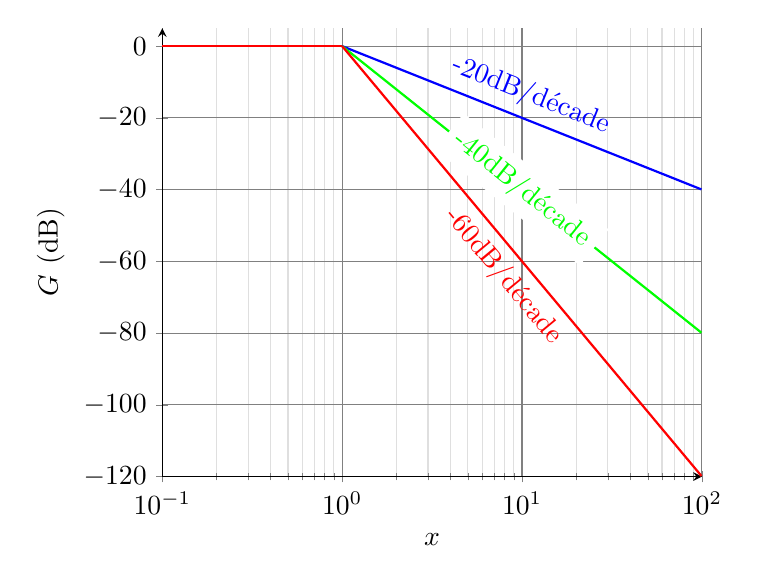
\begin{tikzpicture}[]
    \begin{semilogxaxis}[
        xmin=1e-1, xmax=1e2,
        % xticklabels={\num{e-1}, \num{e3}, \num{e4}},
        % extra x ticks={5e2, 5e3},
        % extra x tick labels={\num{5e2}, \num{5e3}},
        % extra x tick style={grid=minor, grid style={gray!25}, font=\tiny},
        ymin=-120, ymax=5,
        %ytick={-55, -50, ..., -10},
        xlabel={$x$}, ylabel=$G_{\dB}$ (dB),
        axis lines=left,
        grid=both,
        minor grid style={gray!25},
        major grid style={black!50},
        % width=10cm,
        % height=7cm,
        clip=false]
        \addplot[
        domain=1e-1:1,
        smooth, samples=500, red, thick]
        {0};
        \addplot[
        domain=1:1e2,
        smooth, samples=500, blue, thick]
        {-20*log10(\x)}
        node [midway, sloped, above] {\SI{-20}{dB/d\'ecade}};
        \addplot[
        domain=1:1e2,
        smooth, samples=500, green, thick]
        {-40*log10(\x)}
        node [midway, sloped, fill=white] {\SI{-40}{dB/d\'ecade}};
        \addplot[
        domain=1:1e2,
        smooth, samples=500, red, thick]
        {-60*log10(\x)}
        node [midway, sloped, below] {\SI{-60}{dB/d\'ecade}};
        % \draw[thick, dashed]
        % (axis cs:1e-1,-9.5) -|
        % (axis cs:1,-40);
    \end{semilogxaxis}
\end{tikzpicture}
\end{document}
